\begin{table}[tb]
    \centering
    \fontsize{11}{11}
    \small
	% Model Manufacturer Category PLP-Support Capacitor 
    %\begin{tabular}{p{2.4cm}|p{1.3cm}|p{1.2cm}|l}
    %\begin{tabular}{p{2.4cm}|p{2.4cm}|p{2.4cm}|p{2.4cm}|p{2.4cm}}
    \begin{tabular}{|l|l|l|l|}
    %\begin{tabular}{|p{5cm}|l|l|l|}
        % \hline
        % \multirow{4}{*}{{\rotatebox{90}{\parbox{1.2cm}{\centering \footnotesize{Concurrency}}}}} 
		\hline
		\bf{Workload} & \bf{Reqs.} & \bf{Footprint(D)} & \bf{Footprint(M)} \\ \hline \hline
		fileserver & 4965791 & XX & XX \\ \hline 		
		webserver & 15264309 & XX & XX \\ \hline 		
		linkbench & 3412657 & XX & XX \\ \hline 		
		YCSB-00 & 70682260 & XX & XX \\ \hline 		
		YCSB-01 & 58037200 & XX & XX \\ \hline 		
		Systor-16LUN3 & 1200345 & XX & XX \\ \hline 		
		Systor-16LUN4 & 1000701 & XX & XX \\ \hline 		
		Systor-18LUN3 & 1464747 & XX & XX \\ \hline 		
%        Channel & 8x \\ \hline
%        Way & 4x \\ \hline
%        Die & 4x \\ \hline
%        Plane & 4x \\ \hline
%        Page Size & 4KB \\ \hline
%        SSD Capacity & 512GB \\ \hline
    \end{tabular}
    \caption{\textbf{Workload Characteristics.}}
    \label{tab:wk_char}
    % \vspace{-10pt}
\end{table}


\begin{figure*}[!bt]
    \centering{}
    \subfloat[Fileserver]{
        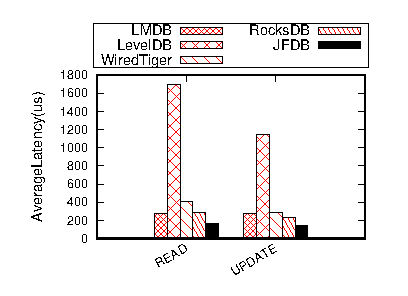
\includegraphics[width=0.24\textwidth]{./ycsb_graph/ycsb_16_a.eps}
	}
    \subfloat[Webserver]{
        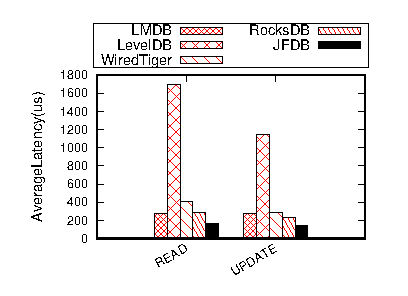
\includegraphics[width=0.24\textwidth]{./ycsb_graph/ycsb_16_a.eps}
	} 
    \subfloat[Linkbench]{
        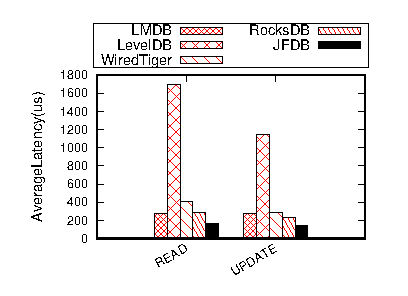
\includegraphics[width=0.24\textwidth]{./ycsb_graph/ycsb_16_a.eps}
	}
	\subfloat[YCSB-00]{
        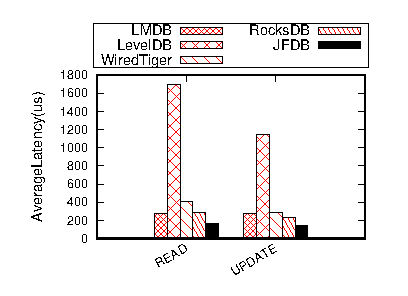
\includegraphics[width=0.24\textwidth]{./ycsb_graph/ycsb_16_a.eps}
	} \\
	\subfloat[YCSB-01]{
        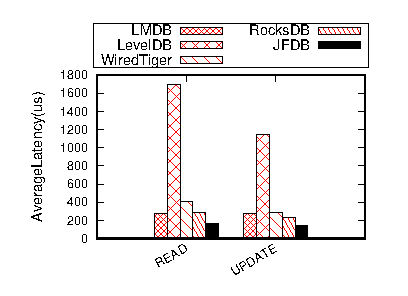
\includegraphics[width=0.24\textwidth]{./ycsb_graph/ycsb_16_a.eps}
	} 
	\subfloat[Systor-16LUN3]{
        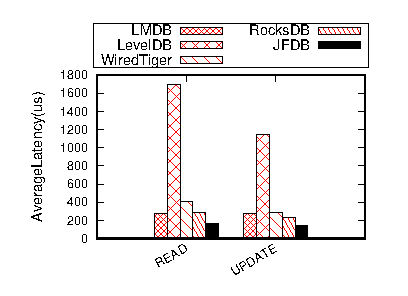
\includegraphics[width=0.24\textwidth]{./ycsb_graph/ycsb_16_a.eps}
	} 
	\subfloat[Systor-16LUN4]{
        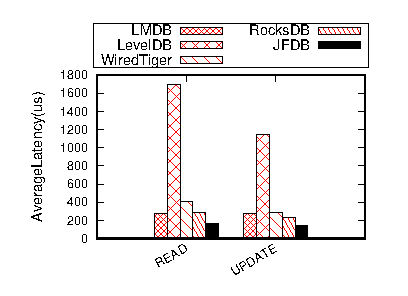
\includegraphics[width=0.24\textwidth]{./ycsb_graph/ycsb_16_a.eps}
	} 
	\subfloat[Systor-18LUN3]{
        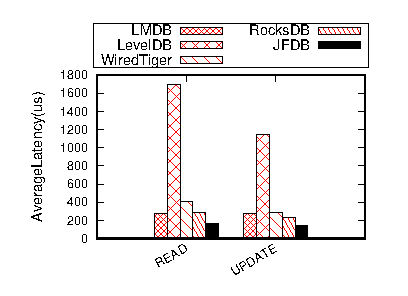
\includegraphics[width=0.24\textwidth]{./ycsb_graph/ycsb_16_a.eps}
	} 

	\caption{\textbf{Hit ratio in protected mapping table pages.}
%		\st{The \texttt{fillrandom} inserts items with random keys for each thread,
%    and the \texttt{overwrite} updates existing values in random order.
%    Both represent a put operation.
%    The \texttt{readrandom} retrieves items randomly,
%    and the \texttt{seekrandom} performs random seeks and queries the next ten items.}
	 }\label{fig_hit_ratio}
\end{figure*} 



\begin{figure*}[!bt]
    \centering{}
    \subfloat[Fileserver]{
        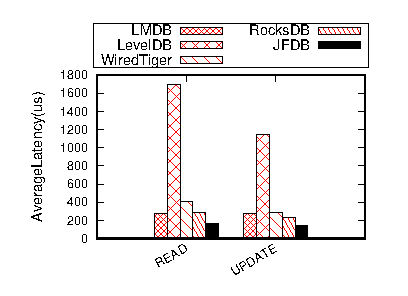
\includegraphics[width=0.24\textwidth]{./ycsb_graph/ycsb_16_a.eps}
	}
    \subfloat[Webserver]{
        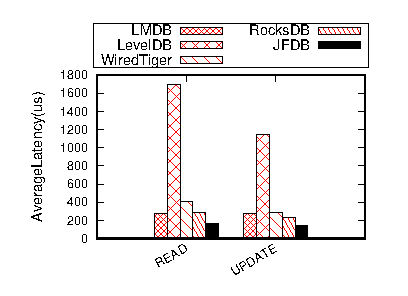
\includegraphics[width=0.24\textwidth]{./ycsb_graph/ycsb_16_a.eps}
	} 
    \subfloat[Linkbench]{
        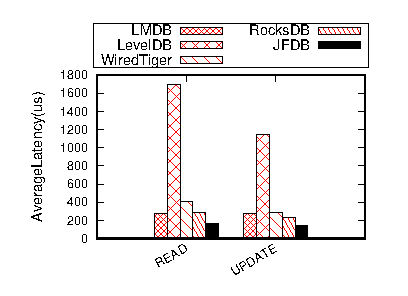
\includegraphics[width=0.24\textwidth]{./ycsb_graph/ycsb_16_a.eps}
	}
	\subfloat[YCSB-00]{
        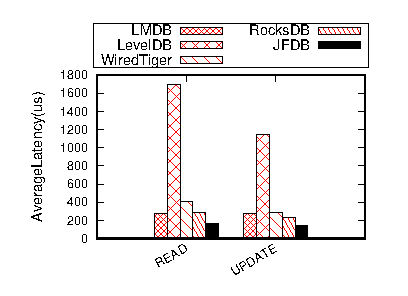
\includegraphics[width=0.24\textwidth]{./ycsb_graph/ycsb_16_a.eps}
	} \\
	\subfloat[YCSB-01]{
        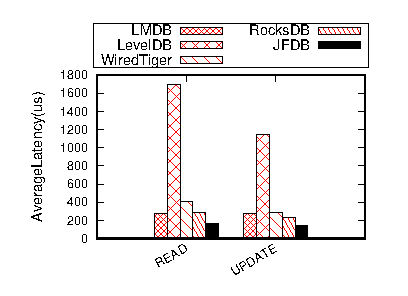
\includegraphics[width=0.24\textwidth]{./ycsb_graph/ycsb_16_a.eps}
	} 
	\subfloat[Systor-16LUN3]{
        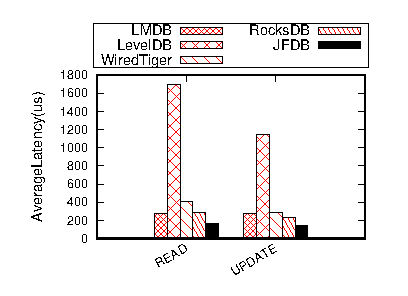
\includegraphics[width=0.24\textwidth]{./ycsb_graph/ycsb_16_a.eps}
	} 
	\subfloat[Systor-16LUN4]{
        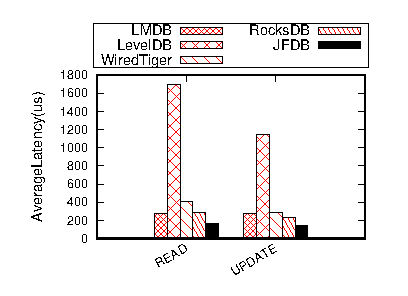
\includegraphics[width=0.24\textwidth]{./ycsb_graph/ycsb_16_a.eps}
	} 
	\subfloat[Systor-18LUN3]{
        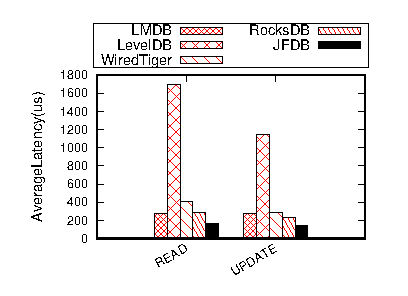
\includegraphics[width=0.24\textwidth]{./ycsb_graph/ycsb_16_a.eps}
	} 

	\caption{\textbf{Write-back traffic of mapping table.}
%		\st{The \texttt{fillrandom} inserts items with random keys for each thread,
%    and the \texttt{overwrite} updates existing values in random order.
%    Both represent a put operation.
%    The \texttt{readrandom} retrieves items randomly,
%    and the \texttt{seekrandom} performs random seeks and queries the next ten items.}
	 }\label{fig_write_traffic}
\end{figure*} 


